\documentclass[10pt]{article}

\usepackage[top=0.8in,bottom=0.8in]{geometry}
\usepackage{amsmath}
\usepackage{amssymb}
\usepackage{graphicx}
\usepackage{tikz}
\usetikzlibrary{positioning}
\usepackage{mathtools}
% Enables font change size in verbatim blocks
\makeatletter
\newcommand{\verbatimfont}[1]{\renewcommand{\verbatim@font}{\ttfamily#1}}
\makeatother
\usepackage{hyperref}
\hypersetup{
    colorlinks=true,
    linkcolor=blue,
    filecolor=magenta,      
    urlcolor=cyan,
}
 
\urlstyle{same}

% Format for answering questions
\newenvironment{answer}
    {\begin{center}
    \begin{tabular}{|p{1\textwidth}|}
    \hline
    }
    { 
    \\\hline
    \end{tabular} 
    \end{center}
    }
 

\begin{document}

\title{CS 4120: Homework 1}
\author{Adam Camilli (aocamilli@wpi.edu)}
\date{\today}
\maketitle

\section*{Problem 1}
Find the least integer k such that $f(n)$ is $O(n^k)$ for each of the following functions. Include values for $c$ and $n_0$ as described in section 3.1, page 47 of the
textbook.
\begin{itemize}
\item $f(n) = 2n^2 + n^3 \log n$
  \begin{answer}
    Using formal definition of $O(n)$, we obtain
    \[\exists c,n_0 \mid 0 \le 2n^2 + n^3 \log n \le c(n^k) \textrm{ for all $n \ge n_0$}\]
    Asymptotically, we can say
    \[ 2n^2 + n^3 \log n \le cn^4, n \ge n_0 \textrm{  ($n_0 \ge $ the largest root of $\pm cn^4 \mp f(n) = 0$)}\]
    but we cannot say 
    \[ 2n^2 + n^3 \log n \le cn^3 \]
    for any $c$ or $n_0$, since asymptotically $\log n > c$.
    Therefore, the least integer is $k = 4$.
  \end{answer}
\item $f(n) = 3n^5 + (\log n)^4$ 
  \begin{answer}
    Using formal definition of $O(n)$, we obtain
    \[\exists c,n_0 \mid 0 \le 3n^5 + (\log n)^4 \le c(n^k) \textrm{ for all $n \ge n_0$}\]
    Asymptotically, we can say
    \[ 3n^5 + (\log n)^4 \le cn^5, c > 3, n \ge n_0 \textrm{ ($n_0 \ge $ the largest root of $\pm cn^5 \mp f(n) = 0$)}  \]
    but we cannot say 
    \[ 3n^5 + (\log n)^4 \le cn^4 \]
    for any $c$ or $n_0$, since asymptotically $n^5 > n^4$.
    Therefore, the least integer is $k = 5$.
  \end{answer}

\newpage

\item $f(n) = \frac{n^4 + n^2 + 1}{n^4 + 1}$
  \begin{answer}
    Using formal definition of $O(n)$, we obtain
    \[\exists c,n_0 \mid 0 \le \frac{n^4 + n^2 + 1}{n^4 + 1} \le c(n^k) \textrm{ for all $n \ge n_0$}\]
    Asymptotically, we can say
    \[ \frac{n^4 + n^2 + 1}{n^4 + 1} \le cn^0, c > 1, n \neq 0\]
    but we cannot say 
    \[ \frac{n^4 + n^2 + 1}{n^4 + 1} \le cn^{-1} , n \neq 0\]
    for any $c$ or $n_0$, since asymptotically $\frac{n^4 + n^2 + 1}{n^4 + 1} > n^{-1}$. Specifically,
    \[ \lim_{n\to\infty}\frac{n^4 + n^2 + 1}{n^4 + 1} = 1 > \lim_{n\to\infty}n^{-1}= 0 \]

    Therefore, the least integer is $k = 0$.
  \end{answer} 

\item $f(n) = \frac{n^3 + 5 \log n}{n^4 + 1}$
  \begin{answer}
    Using formal definition of $O(n)$, we obtain
    \[\exists c,n_0 \mid 0 \le \frac{n^3 + 5 \log n}{n^4 + 1} \le c(n^k) \textrm{ for all $n \ge n_0$}\]
    Asymptotically, we can say
    \[ \frac{n^3 + 5 \log n}{n^4 + 1} \le cn^{-1}, n \neq 0 \ge n_0, \textrm{ ($n_0 \ge $ the root of $\pm cn^{-1} \mp f(n) = 0$)}\]
    but we cannot say 
    \[ \frac{n^3 + 5 \log n}{n^4 + 1} \le cn^{-2} , n \neq 0\]
    for any $c$ or $n_0$, since asymptotically $\frac{n^3 + 5 \log n}{n^4 + 1} > n^{-2}$.

    Therefore, the least integer is $k = -1$.
  \end{answer} 

\end{itemize}

\newpage

\section*{Problem 2}
You have $n$ quarters and a balance. You know that $n-1$ quarters have
the same weight, and one weighs less than the others. Give an algorithm
(in pseudocode) to identify the light quarter which uses the balance only
$\log_{3}n$ times in the worst case.
\begin{answer}
  Assumptions:
  \begin{enumerate}
  \item We can use the balance to measure any amount of coins (gathering etc. costs nothing)
  \item We are given normal weight $W_n$.
  \item The worst case allowed is $\lceil\log_{3}n\rceil$ uses (impossible otherwise).
  \item Removing items from the balance \textbf{does not count as a use}
  \end{enumerate}
  From these assumptions, we develop the following algorithm, using a mathematical generalization for this class of problem (\href{https://en.wikipedia.org/wiki/Balance_puzzle}{source}) that states the minimum number of weightings needed $X$ can be found by 
\[ \frac{3^X-3}{2} = \textrm{ \# of coins}\]
\end{answer}
\begin{center}
  (Pseudocode on next page)
\end{center}
\begin{answer}
\verbatimfont{\scriptsize}%
\begin{verbatim}
/* Given values */
Wn // Normal weight
balance // the state of the balance

/* Returns whether weight is normal */
normalWeight():
  if (balance.weight == Wn*balance.coinsWeighed())
    return true
  else
    return false

/* Remove these coin(s) from scale 
   DOES NOT COUNT AS A USE OF SCALE */
remove(coins):
  //elided

/* A reduced recursive algorithm for an amount of coins that is a power of 3 
   Returns light coin, using exactly log3(coins.size) weighings */
3-algo(coins):     
  if (coins.size <= 3):
    weigh(coins) // ONLY USE OF THE SCALE IN THIS FUNCTION (THIS IF-ELSE BLOCK MUST RETURN)
    if (normalWeight()) // This group of 3 is all normal coins
      return NULL
    else 
      remove(coins[0]) // Arbitrary, could be any of the 3
      if normalWeight() // Must return by this point if size==1
         return coins[0]
      else
         remove(coins[1]) // Arbitrary, could be either of the 2
         if normalWeight()
           return coins[1] // Must return by this point if size == 2
         else // If size was two or one, will have returned 
           return coins[2]
  /* Use this exact same structure with exactly 3 groups of coins. Since coins.size is a 
     power of 3, it is guaranteed to eventually reduce to the if-else block above.
     Since the scale is used only once per call of 3-algo(), this means it will be used exactly 
     log3(coins.size) times! */
  groups = split(coins,coins/3)
  weigh(groups) // ONLY USE OF THE SCALE IN THIS FUNCTION
    if (normalWeight()) // All coins are normal 
      return NULL
    else 
      remove(groups[0]) // Arbitrary, could be any of the 3
      if normalWeight()
         return 3-algo(groups[0])
      else
         remove(groups[1]) // Arbitrary, could be either of the 2
         if normalWeight()
           return 3-algo(groups[1])
         else
           return 3-algo(groups[2])

/* Main algorithm for any number of coins. Essentially, it calculates floor(X) where X is the 
   generalization explained above, and therefore can split N coins into groups of 3^X, 3^(X-1), ...
   This can result in three possible groupings:

   3^X 3^(X-1) ... 3^1       (if coins.size mod 3 == 0) 
   --------> just call 3-algo()
   3^X 3^(X-1) ... 3^0       (if coins.size mod 3 == 1) 
   --------> call 3-algo(), if NULL then last coin (3^0) is light
   3^X 3^(X-1) ... 3^0 3^0   (if coins.size mod 3 == 2) 
   --------> call 3-algo(), just call 3-algo() with last two combined as an "extra" group of two

   In the first two cases, there are exactly floor(log3(coins.size)) uses of the scale. In case 3, however,
   there will be floor(log3(coins.size)) + 1 uses. THIS IS OK, due to our assumption that
   MAX_USES = ceil(log3(coins.size)) */
lightestCoin(coins):
   // Solve generalization ((3^X) - 3)/2 = coins.size for X
   X = floor(log3(2(coins.size) + 3))
   switch(X):
     case (X mod 3 == 0):
       return 3-algo(coins)
     case (X mod 3 == 1):
       if ((result = 3-algo(coins.subArray(coins.size - 1))) != NULL)
         return result
       else 
         return coins[coins.size - 1] // Will be last coin, since arrays counted from 0
     default: // X mod 3 must be 2
       if ((result = 3-algo(coins.subArray(coins.size - 2))) != NULL)
         return result
       else 
         return 3-algo(coins.subArray(coins.size - 2, coins.size)) 
\end{verbatim}
\end{answer}
\section*{Problem 3}
Use the Master Theorem to find the asymptotic solutions for the following recurrences
3
\begin{itemize}
\item $T(n) = 7T(\frac{n}{2}) + n^2$
  \begin{answer}
    Adapting this relation to the general formula
    \[ T(n) = aT\left(\frac{n}{b}\right) + f(N) \]
    we obtain: 
    \begin{gather*}
     a = 7, b = 2 \\
     f(n) = n^2 \rightarrow O(n^c), c = 1\\
     c_{\textrm{crit}} = \log_27 \approx 2.81 \\
     c < c_{\textrm{crit}} \rightarrow \textrm{ CASE 1} \\
   \end{gather*}
   This gives us the solution:
   \[ T(n) = \Theta(n^{\log_27}) \]
  \end{answer}

\item $T(n) = T (\frac{n}{2}) + 1$
    \begin{answer}
    Adapting this relation to the general formula
    \[ T(n) = aT\left(\frac{n}{b}\right) + f(N) \]
    we obtain: 
    \begin{gather*}
     a = 1, b = 2 \\
     f(n) = 1 \rightarrow \Theta(n^clog^kn), c = 0, k = 0\\
     c_{\textrm{crit}} = \log_21 = 0 \\
     c = c_{\textrm{crit}} \rightarrow \textrm{ CASE 2} \\
   \end{gather*}
   This gives us the solution (choose any $k \ge 0$):
   \[ T(n) = \Theta(n^{\log_21}log^{k+1}n) = \Theta(n^0\log^1n = \Theta(n\log n\]
  \end{answer}
\newpage
\item $T(n) = 4T(\frac{n}{2}) + n^3$
  \begin{answer}
    Adapting this relation to the general formula
    \[ T(n) = aT\left(\frac{n}{b}\right) + f(N) \]
    we obtain: 
    \begin{gather*}
     a = 4, b = 2 \\
     f(n) = n^3 \rightarrow \Omega(n^c), c = 3 \\
     c_{\textrm{crit}} = \log_24 = 2 \\
     c > c_{\textrm{crit}} \rightarrow \textrm{ CASE 3} \\
   \end{gather*}
   Since this is case 3, we must additionally satisfy the regularity condition
   \[ af\left(\frac{n}{b}\right) \le kf(n() , k < 1\]
   Using $k = $, we can do so:
   \[ 4\left(\frac{n^3}{2^3}\right) \le kn^3, k = \frac{1}{2} \]
   Therefore $T(n)$ is dominated by splitting term $n^3$, and we obtain asymptotic solution
   \[ T(n) = \Theta(n^3) \]
  \end{answer}
\end{itemize}

\section*{Problem 4}
$A[1...n]$ is a \textbf{sorted} array of \textbf{distinct} integers. We want to decide whether there is an index $i$ where $A[i] = i$.

\begin{itemize}
\item Describe a divide-and-conquer algorithm that solves this problem.
\item Use the Master Theorem to estimate the running time of the algorithm. Your algorithm should run in $O(\log n)$ time
\end{itemize}

\begin{answer}
  Insights:
  \begin{enumerate}
  \item After passing index $i$, we no longer need to check for $A[i] = i$ since $A$ is sorted and distinct. Therefore by simply iterating through array, checking at each index, we achieve linear runtime.
  \item Since $A$ is sorted, if $A[i]$ is found that is greater than $i$ (i.e. $A[2] = 4$) we can skip all following indices that are less than $A[i]$.
  \end{enumerate}

  Consider an array $B$ where 
  \[ B[i] = A[i] -i \]
  Since $A[i] < A[i+1]$ because $A$ is sorted and distinct, 
  \[ B[i] = A[i] - i \le A[i+1] - 1 - i = B[i+1] \]
  An index where $A[i] = i$ corresponds to one where $B[i] = 0$, therefore we can simply binary search for 0 in $B$, an $O(\log n)$ operation.
\end{answer}

\section*{Problem 5}
Suppose you are tossing $m$ balls into $n$ bins. Each ball is equally likely to land in each bin, and the ball tosses are independent. What is the expected number of bins that contain exactly $k$ balls? Use indicator random variables to find the solution.

\begin{answer}
  Let indicator variable $X_i$ be defined as
  \begin{equation*} 
    X_i =
    \begin{cases*}
      1, & \textrm{if $\text{bin}_i$ contains $k$ balls} \\
      0, & \textrm{otherwise}
    \end{cases*}
  \end{equation*}
  Let indicator variable $Y$ equal the number of bins containing $k$ balls:
  \[ Y = X_1 + X_2 + \ldots + X_n \]
  By linearity of expectation,
  \[ E[Y] = E[X_1] + E[X_2] + \ldots + E[X_n] \]
  We now define the probability of a bin $i$ containing $k$ balls. This is a binomial distribution, where $p = \frac{1}{n}$ and $q = \frac{n-1}{n}$. Therefore we need to choose which $k$ of the $m$ balls go into bin $i$, and then which of the other $n-1$ bins will hold the other $m-k$ balls. Divide this by the total number of ways to distribute $m$ balls among $n$ bins:
  \[ P(X_i) = \binom{m}{k}\frac{(n-1)^{m-k}}{n^m} \]
  The expected value of $Y$ can then be derived:
  \[ E[Y] = \sum_{i=1}^nE[X_i] = \binom{m}{k}\frac{(n-1)^{m-k}}{n^{m-1}}\]
\end{answer}

\section*{Problem 6}
Use a recursion tree to determine a good asymptotic upper bound on the recurrence
$T(n) = T(\frac{n}{2}) + n^2$. Use the substitution method to verify your answer.

\begin{answer}
  The rate of increase in the number of subproblems in each recursion $= 1$ \\
  The rate of decrease in subproblem size $= 2$ \\ \\ 
  Therefore in each level of the tree, there is only one node with cost $c\left(\frac{n}{2^i}\right)^2$ at depth $i = 0,1,\ldots \log n$. Total cost:
  \[ T(n) = \sum_{i=0}^{\log n}c\left(\frac{n}{2^i}\right)^2 \le cn^2 \cdot \sum_{i=0}^{\infty}c\left(\frac{1}{4}\right)^i = O(n^2) \textrm{ (since sum is independent)}\]
  Verify using substitution method:
  \[ T(n) = T\left(\frac{n}{2}\right) + n^2 \le d\left(\frac{n}{2}\right)^2 + n^2 = \frac{dn^2}{4} + n^2 \le dn^2, \hspace{1cm} \left(d \ge \frac{4}{3}\right) \]
\end{answer}

\section*{Problem 7}
Using Figure 1 as a model (also can be find in the textbook page 161), illustrate the operation of HEAPSORT on the array
$A=[5, 13, 12, 25, 71, 37, 27, 9, 22]$.
\begin{center}
  \begin{figure}[h!]
    \centering
    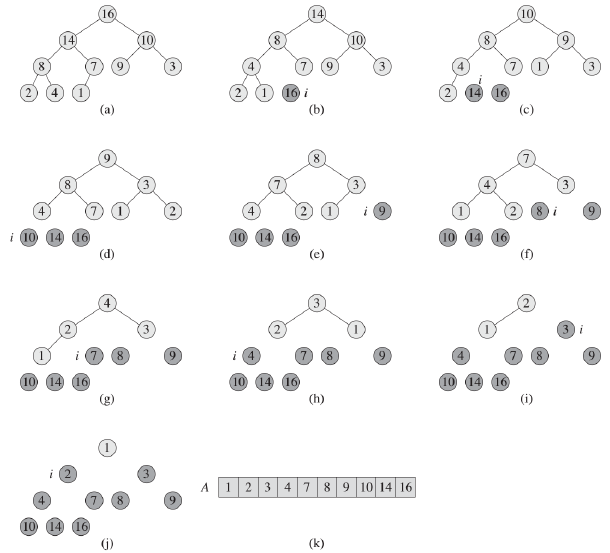
\includegraphics[height=8cm,keepaspectratio]{fig1.png}
  \end{figure}
\end{center}
\begin{answer}
  \begin{minipage}{0.4\textwidth}
    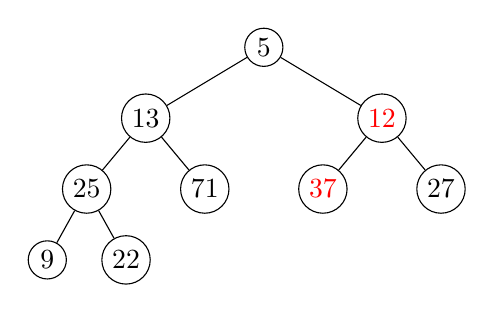
\begin{tikzpicture}[level/.style={level distance=0.9cm,sibling distance=30mm/#1}]
      \node[inner sep=2pt,minimum size=3mm,circle,draw](5){5}
      child{ 
        node[inner sep=2pt,minimum size=3mm,circle,draw](13){13}
        child{ 
          node[inner sep=2pt,minimum size=3mm,circle,draw](25){25}
          child{ 
            node[inner sep=2pt,minimum size=3mm,circle,draw](9){9}
          }
          child{
            node[inner sep=2pt,minimum size=3mm,circle,draw](22){22}
          }
        }
        child{
          node[inner sep=2pt,minimum size=3mm,circle,draw](71){71}
        }
      }
      child{
        node[inner sep=2pt,minimum size=3mm,circle,draw,text=red](12){12}
        child{ 
          node[inner sep=2pt,minimum size=3mm,circle,draw,text=red](37){37}
        }
        child{
          node[inner sep=2pt,minimum size=3mm,circle,draw](27){27}
        }
      };
    \end{tikzpicture}
  \end{minipage}
  $[\ ]\rightarrow$
  \begin{minipage}{0.4\textwidth}
    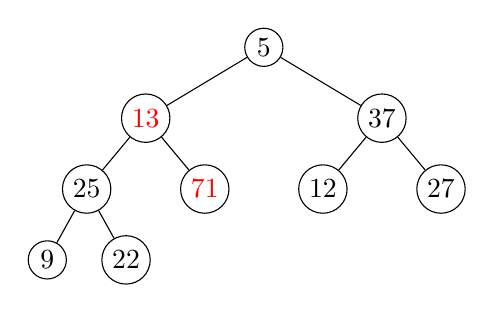
\begin{tikzpicture}[level/.style={level distance=0.9cm,sibling distance=30mm/#1}]
      \node[inner sep=2pt,minimum size=3mm,circle,draw](5){5}
      child{ 
        node[inner sep=2pt,minimum size=3mm,circle,draw,text=red](13){13}
        child{ 
          node[inner sep=2pt,minimum size=3mm,circle,draw](25){25}
          child{ 
            node[inner sep=2pt,minimum size=3mm,circle,draw](9){9}
          }
          child{
            node[inner sep=2pt,minimum size=3mm,circle,draw](22){22}
          }
        }
        child{
          node[inner sep=2pt,minimum size=3mm,circle,draw,text=red](71){71}
        }
      }
      child{
        node[inner sep=2pt,minimum size=3mm,circle,draw](37){37}
        child{ 
          node[inner sep=2pt,minimum size=3mm,circle,draw](12){12}
        }
        child{
          node[inner sep=2pt,minimum size=3mm,circle,draw](27){27}
        }
      };
    \end{tikzpicture}
  \end{minipage} $\rightarrow$
  \\
  \begin{minipage}{0.4\textwidth}
    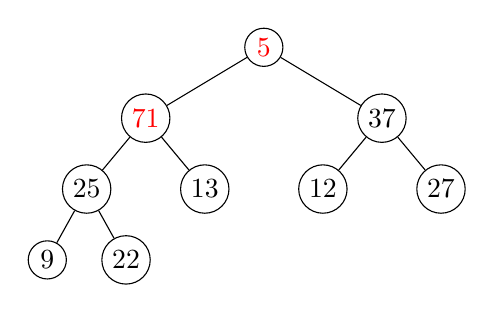
\begin{tikzpicture}[level/.style={level distance=0.9cm,sibling distance=30mm/#1}]
      \node[inner sep=2pt,minimum size=3mm,circle,draw,text=red](5){5}
      child{ 
        node[inner sep=2pt,minimum size=3mm,circle,draw,text=red](71){71}
        child{ 
          node[inner sep=2pt,minimum size=3mm,circle,draw](25){25}
          child{ 
            node[inner sep=2pt,minimum size=3mm,circle,draw](9){9}
          }
          child{
            node[inner sep=2pt,minimum size=3mm,circle,draw](22){22}
          }
        }
        child{
          node[inner sep=2pt,minimum size=3mm,circle,draw](13){13}
        }
      }
      child{
        node[inner sep=2pt,minimum size=3mm,circle,draw](37){37}
        child{ 
          node[inner sep=2pt,minimum size=3mm,circle,draw](12){12}
        }
        child{
          node[inner sep=2pt,minimum size=3mm,circle,draw](27){27}
        }
      };
    \end{tikzpicture}
  \end{minipage}
  $[\ ]\rightarrow$
  \begin{minipage}{0.4\textwidth}
    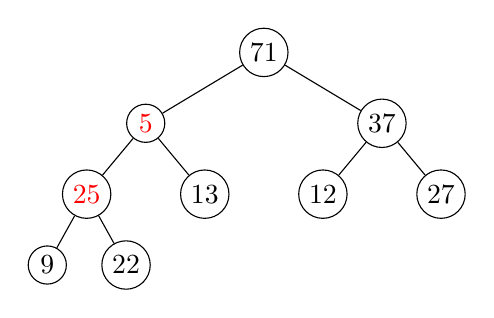
\begin{tikzpicture}[level/.style={level distance=0.9cm,sibling distance=30mm/#1}]
      \node[inner sep=2pt,minimum size=3mm,circle,draw](71){71}
      child{ 
        node[inner sep=2pt,minimum size=3mm,circle,draw,text=red](5){5}
        child{ 
          node[inner sep=2pt,minimum size=3mm,circle,draw,text=red](25){25}
          child{ 
            node[inner sep=2pt,minimum size=3mm,circle,draw](9){9}
          }
          child{
            node[inner sep=2pt,minimum size=3mm,circle,draw](22){22}
          }
        }
        child{
          node[inner sep=2pt,minimum size=3mm,circle,draw](13){13}
        }
      }
      child{
        node[inner sep=2pt,minimum size=3mm,circle,draw](37){37}
        child{ 
          node[inner sep=2pt,minimum size=3mm,circle,draw](12){12}
        }
        child{
          node[inner sep=2pt,minimum size=3mm,circle,draw](27){27}
        }
      };
    \end{tikzpicture}
  \end{minipage} $\rightarrow$
  \\
  \begin{minipage}{0.4\textwidth}
    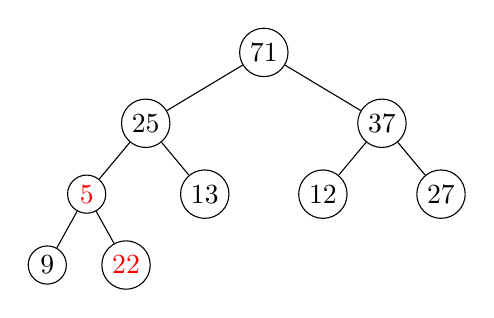
\begin{tikzpicture}[level/.style={level distance=0.9cm,sibling distance=30mm/#1}]
      \node[inner sep=2pt,minimum size=3mm,circle,draw](71){71}
      child{ 
        node[inner sep=2pt,minimum size=3mm,circle,draw](25){25}
        child{ 
          node[inner sep=2pt,minimum size=3mm,circle,draw,text=red](5){5}
          child{ 
            node[inner sep=2pt,minimum size=3mm,circle,draw](9){9}
          }
          child{
            node[inner sep=2pt,minimum size=3mm,circle,draw,text=red](22){22}
          }
        }
        child{
          node[inner sep=2pt,minimum size=3mm,circle,draw](13){13}
        }
      }
      child{
        node[inner sep=2pt,minimum size=3mm,circle,draw](37){37}
        child{ 
          node[inner sep=2pt,minimum size=3mm,circle,draw](12){12}
        }
        child{
          node[inner sep=2pt,minimum size=3mm,circle,draw](27){27}
        }
      };
    \end{tikzpicture}
  \end{minipage}
  $[\ ]\rightarrow$
  \begin{minipage}{0.4\textwidth}
    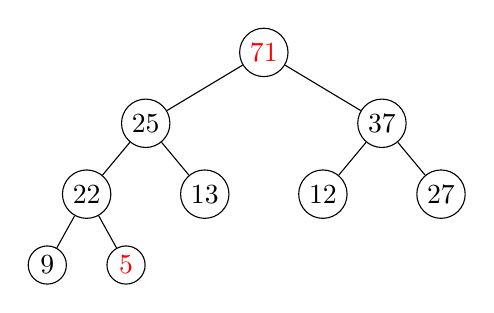
\begin{tikzpicture}[level/.style={level distance=0.9cm,sibling distance=30mm/#1}]
      \node[inner sep=2pt,minimum size=3mm,circle,draw,text=red](71){71}
      child{ 
        node[inner sep=2pt,minimum size=3mm,circle,draw](25){25}
        child{ 
          node[inner sep=2pt,minimum size=3mm,circle,draw](22){22}
          child{ 
            node[inner sep=2pt,minimum size=3mm,circle,draw](9){9}
          }
          child{
            node[inner sep=2pt,minimum size=3mm,circle,draw,text=red](5){5}
          }
        }
        child{
          node[inner sep=2pt,minimum size=3mm,circle,draw](13){13}
        }
      }
      child{
        node[inner sep=2pt,minimum size=3mm,circle,draw](37){37}
        child{ 
          node[inner sep=2pt,minimum size=3mm,circle,draw](12){12}
        }
        child{
          node[inner sep=2pt,minimum size=3mm,circle,draw](27){27}
        }
      };
    \end{tikzpicture}
  \end{minipage} $\rightarrow$
\end{answer}
\newpage
\begin{answer}
    \begin{minipage}{0.4\textwidth}
    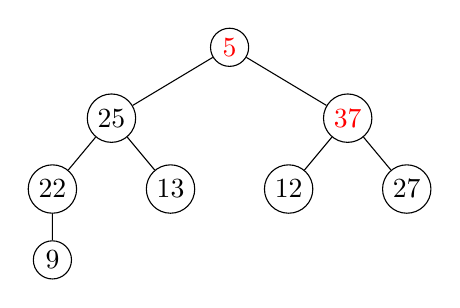
\begin{tikzpicture}[level/.style={level distance=0.9cm,sibling distance=30mm/#1}]
      \node[inner sep=2pt,minimum size=3mm,circle,draw,text=red](5){5}
      child{ 
        node[inner sep=2pt,minimum size=3mm,circle,draw](25){25}
        child{
          node[inner sep=2pt,minimum size=3mm,circle,draw](22){22}
          child{ 
          node[inner sep=2pt,minimum size=3mm,circle,draw](9){9}
          }
        }        
        child{
          node[inner sep=2pt,minimum size=3mm,circle,draw](13){13}
        }
      }
      child{
        node[inner sep=2pt,minimum size=3mm,circle,draw,text=red](37){37}
        child{ 
          node[inner sep=2pt,minimum size=3mm,circle,draw](12){12}
        }
        child{
          node[inner sep=2pt,minimum size=3mm,circle,draw](27){27}
        }
      };
    \end{tikzpicture}
  \end{minipage}
  $[71]\rightarrow$
  \begin{minipage}{0.4\textwidth}
    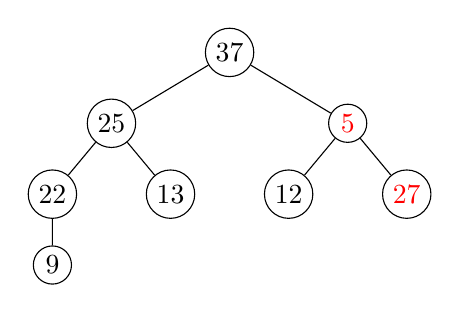
\begin{tikzpicture}[level/.style={level distance=0.9cm,sibling distance=30mm/#1}]
      \node[inner sep=2pt,minimum size=3mm,circle,draw](37){37}
      child{ 
        node[inner sep=2pt,minimum size=3mm,circle,draw](25){25}
        child{
          node[inner sep=2pt,minimum size=3mm,circle,draw](22){22}
          child{ 
          node[inner sep=2pt,minimum size=3mm,circle,draw](9){9}
          }
        }        
        child{
          node[inner sep=2pt,minimum size=3mm,circle,draw](13){13}
        }
      }
      child{
        node[inner sep=2pt,minimum size=3mm,circle,draw,text=red](5){5}
        child{ 
          node[inner sep=2pt,minimum size=3mm,circle,draw](12){12}
        }
        child{
          node[inner sep=2pt,minimum size=3mm,circle,draw,text=red](27){27}
        }
      };
    \end{tikzpicture}
  \end{minipage} $\rightarrow$
  \\
  \begin{minipage}{0.4\textwidth}
    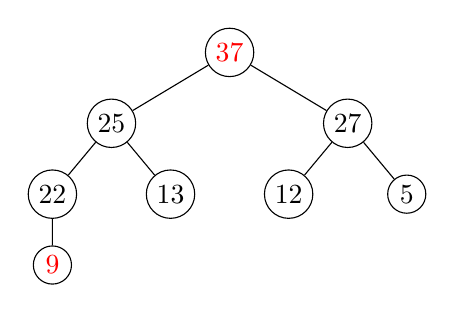
\begin{tikzpicture}[level/.style={level distance=0.9cm,sibling distance=30mm/#1}]
      \node[inner sep=2pt,minimum size=3mm,circle,draw,text=red](37){37}
      child{ 
        node[inner sep=2pt,minimum size=3mm,circle,draw](25){25}
        child{
          node[inner sep=2pt,minimum size=3mm,circle,draw](22){22}
          child{ 
          node[inner sep=2pt,minimum size=3mm,circle,draw,text=red](9){9}
          }
        }        
        child{
          node[inner sep=2pt,minimum size=3mm,circle,draw](13){13}
        }
      }
      child{
        node[inner sep=2pt,minimum size=3mm,circle,draw](27){27}
        child{ 
          node[inner sep=2pt,minimum size=3mm,circle,draw](12){12}
        }
        child{
          node[inner sep=2pt,minimum size=3mm,circle,draw](5){5}
        }
      };
    \end{tikzpicture}
  \end{minipage} 
  $[37,71]\rightarrow$
  \begin{minipage}{0.4\textwidth}
    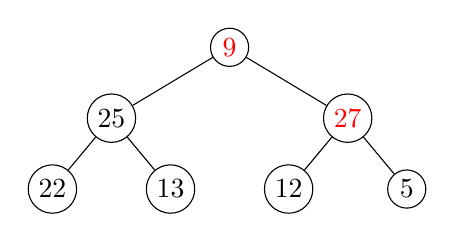
\begin{tikzpicture}[level/.style={level distance=0.9cm,sibling distance=30mm/#1}]
      \node[inner sep=2pt,minimum size=3mm,circle,draw,text=red](9){9}
      child{ 
        node[inner sep=2pt,minimum size=3mm,circle,draw](25){25}
        child{
          node[inner sep=2pt,minimum size=3mm,circle,draw](22){22}
        }        
        child{
          node[inner sep=2pt,minimum size=3mm,circle,draw](13){13}
        }
      }
      child{
        node[inner sep=2pt,minimum size=3mm,circle,draw,text=red](27){27}
        child{ 
          node[inner sep=2pt,minimum size=3mm,circle,draw](12){12}
        }
        child{
          node[inner sep=2pt,minimum size=3mm,circle,draw](5){5}
        }
      };
    \end{tikzpicture}
  \end{minipage} $\rightarrow$
  \\
  \begin{minipage}{0.4\textwidth}
    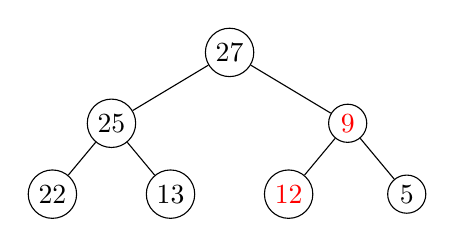
\begin{tikzpicture}[level/.style={level distance=0.9cm,sibling distance=30mm/#1}]
      \node[inner sep=2pt,minimum size=3mm,circle,draw](27){27}
      child{ 
        node[inner sep=2pt,minimum size=3mm,circle,draw](25){25}
        child{
          node[inner sep=2pt,minimum size=3mm,circle,draw](22){22}
        }        
        child{
          node[inner sep=2pt,minimum size=3mm,circle,draw](13){13}
        }
      }
      child{
        node[inner sep=2pt,minimum size=3mm,circle,draw,text=red](9){9}
        child{ 
          node[inner sep=2pt,minimum size=3mm,circle,draw,text=red](12){12}
        }
        child{
          node[inner sep=2pt,minimum size=3mm,circle,draw](5){5}
        }
      };
    \end{tikzpicture}
  \end{minipage} 
  $[37,71]\rightarrow$
  \begin{minipage}{0.4\textwidth}
    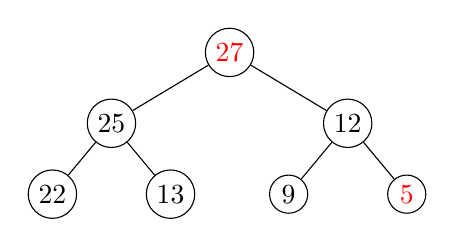
\begin{tikzpicture}[level/.style={level distance=0.9cm,sibling distance=30mm/#1}]
      \node[inner sep=2pt,minimum size=3mm,circle,draw,text=red](27){27}
      child{ 
        node[inner sep=2pt,minimum size=3mm,circle,draw](25){25}
        child{
          node[inner sep=2pt,minimum size=3mm,circle,draw](22){22}
        }        
        child{
          node[inner sep=2pt,minimum size=3mm,circle,draw](13){13}
        }
      }
      child{
        node[inner sep=2pt,minimum size=3mm,circle,draw](12){12}
        child{ 
          node[inner sep=2pt,minimum size=3mm,circle,draw](9){9}
        }
        child{
          node[inner sep=2pt,minimum size=3mm,circle,draw,text=red](5){5}
        }
      };
    \end{tikzpicture}
  \end{minipage} $\rightarrow$
  \\ \\
  \begin{minipage}{0.38\textwidth}
    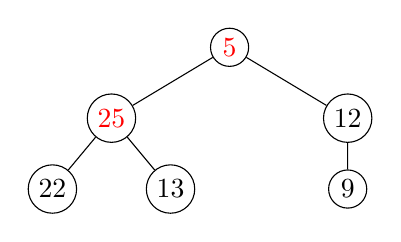
\begin{tikzpicture}[level/.style={level distance=0.9cm,sibling distance=30mm/#1}]
      \node[inner sep=2pt,minimum size=3mm,circle,draw,text=red](5){5}
      child{ 
        node[inner sep=2pt,minimum size=3mm,circle,draw,text=red](25){25}
        child{
          node[inner sep=2pt,minimum size=3mm,circle,draw](22){22}
        }        
        child{
          node[inner sep=2pt,minimum size=3mm,circle,draw](13){13}
        }
      }
      child{
        node[inner sep=2pt,minimum size=3mm,circle,draw](12){12}
        child{ 
          node[inner sep=2pt,minimum size=3mm,circle,draw](9){9}
        }
      };
    \end{tikzpicture}
  \end{minipage}
  $[27,37,71]\rightarrow$
  \begin{minipage}{0.4\textwidth}
    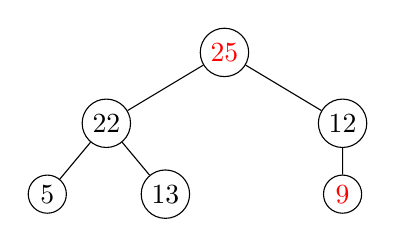
\begin{tikzpicture}[level/.style={level distance=0.9cm,sibling distance=30mm/#1}]
      \node[inner sep=2pt,minimum size=3mm,circle,draw,text=red](25){25}
      child{ 
        node[inner sep=2pt,minimum size=3mm,circle,draw](22){22}
        child{
          node[inner sep=2pt,minimum size=3mm,circle,draw](5){5}
        }        
        child{
          node[inner sep=2pt,minimum size=3mm,circle,draw](13){13}
        }
      }
      child{
        node[inner sep=2pt,minimum size=3mm,circle,draw](12){12}
        child{ 
          node[inner sep=2pt,minimum size=3mm,circle,draw,text=red](9){9}
        }
      };
    \end{tikzpicture}
  \end{minipage} $\rightarrow$
  \\ \\
  \begin{minipage}{0.33\textwidth}
    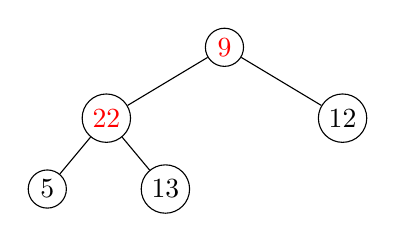
\begin{tikzpicture}[level/.style={level distance=0.9cm,sibling distance=30mm/#1}]
      \node[inner sep=2pt,minimum size=3mm,circle,draw,text=red](9){9}
      child{ 
        node[inner sep=2pt,minimum size=3mm,circle,draw,text=red](22){22}
        child{
          node[inner sep=2pt,minimum size=3mm,circle,draw](5){5}
        }        
        child{
          node[inner sep=2pt,minimum size=3mm,circle,draw](13){13}
        }
      }
      child{
        node[inner sep=2pt,minimum size=3mm,circle,draw](12){12}
      };
    \end{tikzpicture}
  \end{minipage}
  $[25,27,37,71]\rightarrow$
  \begin{minipage}{0.4\textwidth}
    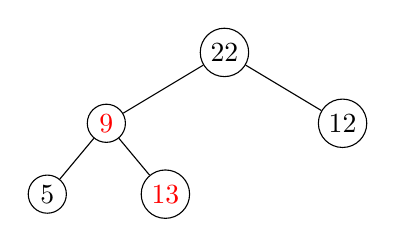
\begin{tikzpicture}[level/.style={level distance=0.9cm,sibling distance=30mm/#1}]
      \node[inner sep=2pt,minimum size=3mm,circle,draw](22){22}
      child{ 
        node[inner sep=2pt,minimum size=3mm,circle,draw,text=red](9){9}
        child{
          node[inner sep=2pt,minimum size=3mm,circle,draw](5){5}
        }        
        child{
          node[inner sep=2pt,minimum size=3mm,circle,draw,text=red](13){13}
        }
      }
      child{
        node[inner sep=2pt,minimum size=3mm,circle,draw](12){12}
      };
    \end{tikzpicture}
  \end{minipage} $\rightarrow$
  \\ \\
  \begin{minipage}{0.30\textwidth}
    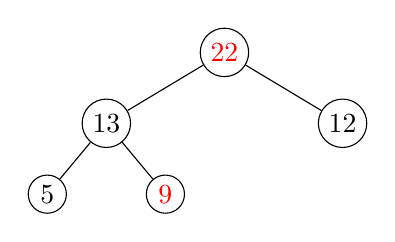
\begin{tikzpicture}[level/.style={level distance=0.9cm,sibling distance=30mm/#1}]
      \node[inner sep=2pt,minimum size=3mm,circle,draw,text=red](22){22}
      child{ 
        node[inner sep=2pt,minimum size=3mm,circle,draw](13){13}
        child{
          node[inner sep=2pt,minimum size=3mm,circle,draw](5){5}
        }        
        child{
          node[inner sep=2pt,minimum size=3mm,circle,draw,text=red](9){9}
        }
      }
      child{
        node[inner sep=2pt,minimum size=3mm,circle,draw](12){12}
      };
    \end{tikzpicture}
  \end{minipage}
  $[22,25,27,37,71]\rightarrow$
  \begin{minipage}{0.4\textwidth}
    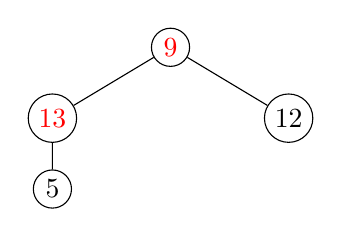
\begin{tikzpicture}[level/.style={level distance=0.9cm,sibling distance=30mm/#1}]
      \node[inner sep=2pt,minimum size=3mm,circle,draw,text=red](9){9}
      child{ 
        node[inner sep=2pt,minimum size=3mm,circle,draw,text=red](13){13}
        child{
          node[inner sep=2pt,minimum size=3mm,circle,draw](5){5}
        }        
      }
      child{
        node[inner sep=2pt,minimum size=3mm,circle,draw](12){12}
      };
    \end{tikzpicture}
  \end{minipage} $\rightarrow$
  \\ \\
  \begin{minipage}{0.27\textwidth}
    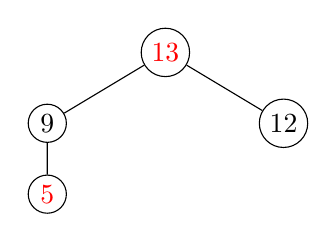
\begin{tikzpicture}[level/.style={level distance=0.9cm,sibling distance=30mm/#1}]
      \node[inner sep=2pt,minimum size=3mm,circle,draw,text=red](13){13}
      child{ 
        node[inner sep=2pt,minimum size=3mm,circle,draw](9){9}
        child{
          node[inner sep=2pt,minimum size=3mm,circle,draw,text=red](5){5}
        }        
      }
      child{
        node[inner sep=2pt,minimum size=3mm,circle,draw](12){12}
      };
    \end{tikzpicture}
  \end{minipage}
  $[13,22,25,27,37,71]\rightarrow$
  \begin{minipage}{0.40\textwidth}
    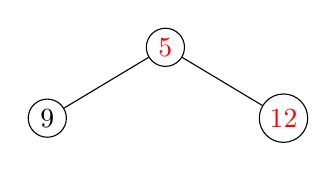
\begin{tikzpicture}[level/.style={level distance=0.9cm,sibling distance=30mm/#1}]
      \node[inner sep=2pt,minimum size=3mm,circle,draw,text=red](5){5}
      child{ 
        node[inner sep=2pt,minimum size=3mm,circle,draw](9){9}
      }
      child{
        node[inner sep=2pt,minimum size=3mm,circle,draw,text=red](12){12}
      };
    \end{tikzpicture}
  \end{minipage} $\rightarrow$
  \\ \\ 
  \begin{minipage}{0.3\textwidth}
    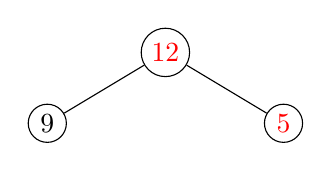
\begin{tikzpicture}[level/.style={level distance=0.9cm,sibling distance=30mm/#1}]
      \node[inner sep=2pt,minimum size=3mm,circle,draw,text=red](12){12}
      child{ 
        node[inner sep=2pt,minimum size=3mm,circle,draw](9){9}
      }
      child{
        node[inner sep=2pt,minimum size=3mm,circle,draw,text=red](5){5}
      };
    \end{tikzpicture}
  \end{minipage}
   $\rightarrow$
  \begin{minipage}{0.1\textwidth}
    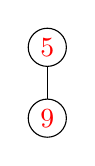
\begin{tikzpicture}[level/.style={level distance=0.9cm,sibling distance=30mm/#1}]
      \node[inner sep=2pt,minimum size=3mm,circle,draw,text=red](5){5}
      child{ 
        node[inner sep=2pt,minimum size=3mm,circle,draw,text=red](9){9}
      };
    \end{tikzpicture}
  \end{minipage} 
  $\rightarrow \ [5,9,12,13,22,25,27,37,71]$
\end{answer}

\section*{Problem 8}
Using QUICKSORT to sort the array $A=[5, 13, 12, 25, 71, 37]$. You just need to show the result after each round. Here is a example for $A=[2, 8, 7, 1, 3, 5, 6, 4]$, suppose you pick the last element in a region as its pivot:

round 1: region=$A$, result=$[2, 1, 3, 4, 7, 5, 6, 8]$

round 2: region$_1$=$[2, 1, 3]$, region$_2$=$[7, 5, 6, 8]$, result=$[2, 1, 3, 4, 7, 5, 6, 8]$. 

round 3: region$_1$=$[2,1]$, region$_2$=$[7, 5, 6]$, result=$[1, 2, 3, 4, 5, 6, 7, 8]$.

The fig 2 shows the the detail operations during the round 1.

%\input{fig_quicksort}

\section*{Problem 9}
The input is two sets $S1$ and $S2$ containing $n$ real numbers in total, and a real number $x$.

(a) Find a O($n$log$n$) time algorithm that determines whether there exists an element from $S1$ and an element from $S2$ whose sum is exactly $x$.

(b) Suppose now that the two sets are given in sorted order. Find a O($n$)-time algorithm solving this problem.

You can either show pseudo code or describe it in English.

\section*{Problem 10}
Show that $2n-1$ comparisons are necessary in the worst case to merge
two sorted lists containing $n$ elements each.


%If you want centered math on its own line, you can use a slash and square bracket.\\
%\[
%\left \{
%\sum\limits_{k=1}^\infty l(I_k):A\subseteq \bigcup_{k=1}^\infty \{I_k\}
%\right \}
%\]
%The left and right commands make the brackets get as big as we need them to be.
%
%\clearpage %Gives us a page break before the next section. Optional.

\section*{Problem 11 $\star$}
Show an example that COUNTING SORT can be slower than any comparison sorts you have learned. (This problem is for practice,  but will not be counted towards the grade)


\end{document}
